% LaTeX resume using res.cls
\documentclass[line,margin]{res}
%\usepackage{helvetica} % uses helvetica postscript font (download helvetica.sty)
%\usepackage{newcent}   % uses new century schoolbook postscript font

\oddsidemargin -.5in
\evensidemargin -.5in
\addtolength{\textwidth}{1.0in}
%\usepackage[letterpaper, margin=0.5in]{geometry}

\usepackage{hyperref}

\newcommand{\superscript}[1]{\ensuremath{^{\textrm{#1}}}}
\newcommand{\subscript}[1]{\ensuremath{_{\textrm{#1}}}}

\newcommand{\namestyle}[1]{\underline{\bf #1 }}

% Define some styles we use
\newcommand{\titlestyle}[1]{{\bf #1}}
\newcommand{\placestyle}[1]{\footnotesize $\cdot$\ \ {\emph{#1}}}
\newcommand{\datestyle}[1]{{\tiny \dotfill} {\small (#1)}}

\renewcommand{\labelitemi}{{\small $\bullet$}}
\renewcommand{\labelitemii}{--}
\renewcommand{\labelitemiii}{$\circ$}
\renewcommand{\labelitemiv}{$\diamond$}

\usepackage{graphicx}

\usepackage{enumitem}
\setitemize{itemsep=0.5pt,topsep=0pt,parsep=0pt,partopsep=0pt}
\setenumerate{itemsep=0.5pt,topsep=0pt,parsep=0pt,partopsep=0pt}

\usepackage{tikz}
\usetikzlibrary{positioning}

\usepackage{microtype}
\usepackage{times}

\begin{document}

\begin{tikzpicture}[remember picture, overlay]
  \node[rectangle] at (14.15, -2.8)
   {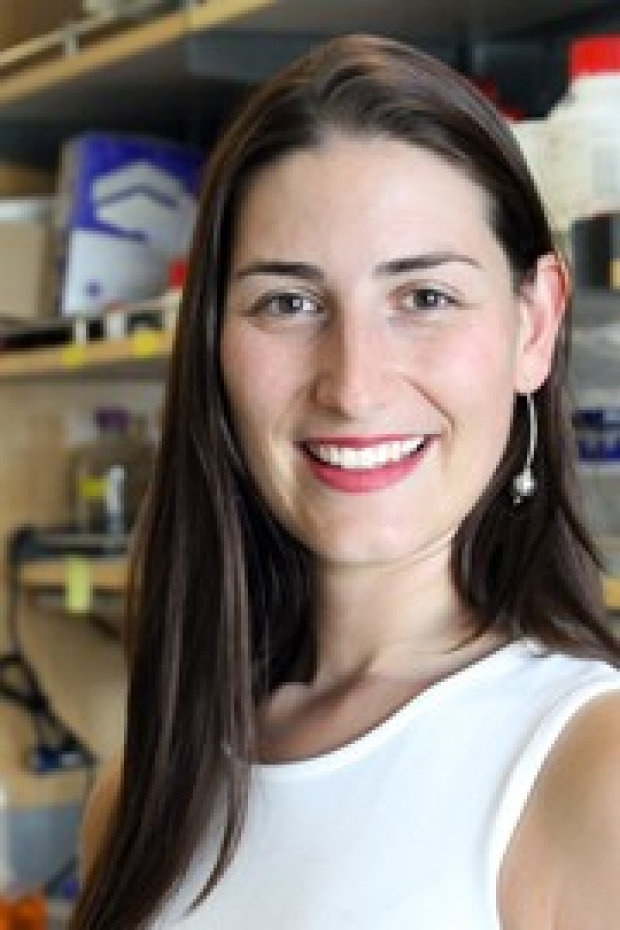
\includegraphics[width=3cm]{cv-image.jpg}
  };
\end{tikzpicture}

\vspace{-0.55in}
\name{Viola Caretti M.D. Ph.D.}
% \address used twice to have two lines of address
\address{+1 (650) 704-5020}
\address{viola@caretti.md}

\begin{resume}

\section{OBJECTIVE}
\begin{itemize}
\item {\small To find a cure for brain cancer in children, with focus on DIPG}
\end{itemize}

\section{HIGHLIGHTS \\ OF \\ QUALIFICATIONS}
\begin{itemize}
  \item {\small {\bf Resident in Pediatric Neurology:} Baylor Texas Children's Hospital}
  \item {\small {\bf California Medical License}}
  \item {\small {\bf Former Resident in Pediatric Neurology:} Stanford Medicine}
  \item {\small {\bf Former Postdoctoral Fellow} in Postnatal Neurodevelopment at Stanford}
  \item {\small {\bf PhD} in Pediatric Neuro-Oncology}
  \item {\small Licensed {\bf Doctor of Medicine} in the EU}
  \item {\small {\bf First authorship} on 10 published manuscripts}
  \item {\small Began a {\bf novel line of research} on DIPG}
  \item {\small {\bf Setup \emph{in vivo} work} in the NRG}
  \item {\small Numerous {\bf grants}, {\bf awards} and {\bf scholarships}}
  \item {\small Extensive {\bf mentoring}, international, and {\bf volunteer} experience}
\end{itemize}

\section{WORK \\ AUTHORIZATION}
\begin{itemize}
\item Permanent Resident (Green Card Holder)
\end{itemize}

\vspace{15pt}
\section{EDUCATION}
\begin{itemize}
\item {
  \titlestyle{Baylor Texas Children's Hospital} \datestyle{August 2019 - present} \\
  { \placestyle{Houston, TX, USA} } \\
  Pediatric Neurology Resident
}
\item {
  \titlestyle{Stanford University School of Medicine} \datestyle{June 2017 -- June 2019} \\
  { \placestyle{Stanford, CA, USA} } \\
  Pediatric Neurology Resident
}
\item {
  \titlestyle{Stanford University} \datestyle{October 2012 -- May 2017} \\
  { \placestyle{Stanford, CA, USA} } \\
  Monje Lab \\
  Postdoctoral Fellow: \emph{``Neuro-glial Interactions in the Glioma Microenvironment''} \\
  Stanford Optogentics Innovation Laboratory Course \datestyle{January 2013}
}
\item {
  \titlestyle{Cancer Center Amsterdam, VUmc} \datestyle{May 2008 -- July 2012} \\
  { \placestyle{Amsterdam, The Netherlands} } \\
  Neuro-Oncology Research Group (NRG), VU University Medical Center (VUmc) \\
  Ph.D. Project: \emph{``Diffuse intrinsic pontine gliomas: towards new treatment strategies''}
%  Course: {Laboratory Animal Science} \datestyle{June 2008} \\
%  Course: {Working with Radioactivity} \datestyle{April 2009}
}
\item {
  \titlestyle{Bicocca University of Medicine} \datestyle{October 2000 -- March 2007} \\
  { \placestyle{Milan, Italy} } \\
  Degree: Doctor of Medicine \\
  Thesis: {\small ``Non-dopaminergic systems in Parkinson's Disease: an [\superscript{123}I]$\beta$-CIT SPECT Study''} \\
  \emph{Student Council Representative to the Medicine Faculty} \datestyle{2003 -- 2004}
}
\item {
  \titlestyle{Erasmus Project} \datestyle{March -- December 2006} \\
  { \placestyle{Amsterdam, The Netherlands} } \\
  \emph{Experimental medical thesis internship} at the VUmc (Neurology Department)
}
\item {
  \titlestyle{Impington Village College} \datestyle{September 1998 -- May 2000} \\
  { \placestyle{Cambridge, United Kingdom} } \\
  International Baccalaureate \\
  Ranked 1\superscript{st} among all foreign students and 2\superscript{nd} in the graduating class.
}
\item {
  \titlestyle{Tito Livio Liceum} \datestyle{1994 -- 1998} \\
  { \placestyle{Milan, Italy} } \\
  Classical Studies including Greek and Latin
}
\end{itemize}

\newpage
\section{GRANTS \\ \& \\ FELLOWSHIPS}
\begin{itemize}
  \item \emph{Lyla Nsouli foundation} Brain Cancer Research Grant \datestyle{2015}
  \item \emph{Bear Necessities} Pediatric Cancer Foundation fellowship \datestyle{2014}
  \item \emph{Child Health ResearchInstitute (CHRI)} Grant Support Award \datestyle{2013}
  \item \emph{Deans Postdoctoral Fellowship} (Stanford University) \datestyle{2013}
  \item \emph{American Italian Cancer Foundation (AICF)} fellowship (not accepted) \datestyle{2013}
\end{itemize}

\section{PUBLICATIONS}
\vspace{-0.75pt}
{\footnotesize
\begin{enumerate}
\item M.H.A. Jansen*, T. Lagerweij*, A.C.P. Sewing*, D.J. Vugts, D.G. van Vuurden, C.F.M. Molthoff, \namestyle{V. Caretti}, S.J.E. Veringa, N. Petersen, A.M. Carcaboso, D.P. Noske, W.P. Vandertop, P. Wesseling, G.A.M.S. van Dongen, G.J.L. Kaspers, E. Hulleman. Bevacizumab targeting diffuse intrinsic pontine glioma: results of 89Zr-bevacizumab PET imaging in brain tumor models. \emph{Mol Cancer Ther} (Sept 2016). 15(9):2166-74.
\item H.S. Venkatesh*, T.B. Johung*, \namestyle{V. Caretti*}, A. Noll, Y. Tang, S. Nagaraja, E.M. Gibson, C.W. Mount, J. Polepalli, S.S. Mitra, P.J. Woo, R.C. Malenka, H. Vogel, M. Bredel, P. Mallick, M. Monje. Neuronal Activity Promotes Glioma Growth through Neuroligin-3 Secretion. \emph{Cell} (May 2015). 161(4): 803–816.
\item A.C.P. Sewing*, \namestyle{V. Caretti*}, T. Lagerweij*, P. Schellen, M.H.A. Jansen, D.G. van Vuurden, S. Idema, C.F. Molthoff, W.P. Vandertop, G.J.L. Kaspers, D.P. Noske, E. Hulleman. Convection enhanced delivery of carmustine to the murine brainstem: A feasibility study. \emph{J Neurosci Methods} (Dec 2014). 238:88-94.
\item \namestyle{V. Caretti*}, M. Bugiani*, M. Freret, P. Schellen, M.H.A. Jansen, D.G. van Vuurden, G.J.L. Kaspers, PG Fisher, E Hulleman, P. Wesseling, H Vogel, M Monje. Subventricular spread of diffuse intrinsic pontine glioma. \emph{Acta Neuropathol} (Oct 2014). 128(4):605-7.
\item \namestyle{V. Caretti}, C. Sewing, T. Lagerweij, P. Schellen, M. Bugiani, M.H.A. Jansen, D.G. van Vuurden, A.C. Navis, I. Horsman, P. Wesseling, W.P. Vandertop, D.P. Noske, G.J.L. Kaspers, E. Hulleman, H. Vogel, M. Monje*, T. Wurdinger*. Human pontine glioma cells can induce murine tumors. \emph{Acta Neuropathol} (Apr 2014). 127(6):897-909.
\item E. Giovannetti, Q.Wang, A. Avan, N. Funel, E. Galvani, T. Lagerweij, D. Chiasserini, J.H. Lee, \namestyle{V. Caretti}, A. van der Velde, U. Boggi, Y. Wang, E. Vasile, G.J .Peters, T. Wurdinger, G. Giaccone. Role of CYB5A in pancreatic cancer prognosis and autophagy modulation. \emph{JNCI} (Jan 2014). 106(1):djt346.
\item A. Avan*, \namestyle{V. Caretti*}, N. Funel*, E. Galvani, M. Maftouh, R.J. Honeywell, T. Lagerweij, O.V. Tellingen, D. Campani, D. Fuchs, H.M. Verheul, G.J .Schuurhuis, U. Boggi, G.J. Peters, T. Wrdinger, E. Giovannetti. Crizotinib inhibits metabolic inactivation of gemcitabine in c-Met-driven pancreatic carcinoma. \emph{Cancer Res} (Nov 2015). 73(22):6745-56.
\item \namestyle{V. Caretti*}, L. Hiddingh*, T. Lagerweij, P. Schellen, P.W. Koken, E. Hulleman, D. van Vuurden, W.P. Vandertop, G. Kaspers, D.P. Noske, T. Wurdinger. WEE1 Kinase Inhibition Enhances the Radiation Response of Diffuse Intrinsic Pontine Gliomas. \emph{Mol Cancer Ther} (Feb 2013). 12(2):141-50.
\item \namestyle{V. Caretti*}, M.H.A. Jansen*, D.G. van Vuurden, T. Lagerweij, M. Bugiani, I. Horsman, H. Wessels, P. van der Valk, J. Cloos, D.P. Noske, W.P. Vandertop, P. Wesseling, T. Wurdinger, E. Hulleman, G. Kaspers. Implementation of a Multi-Institutional Diffuse Intrinsic Pontine Glioma Autopsy Protocol and Characterization of a Primary Cell Culture. \emph{Neuropathol Appl Neurobiol} (Jun 2013). 39(4):426-36.
\item \namestyle{V. Caretti}, D.P Noske, W.P. Vandertop, G. Kaspers, T. Wurdinger. Pioneering Preclinical Research in Diffuse Intrinsic Pontine Glioma: Towards New Treatment Strategies. \emph{PhD Thesis} (July 2012).
\item S. Idema, \namestyle{V. Caretti}, M. Lamfers, V. van Beusechem, D. Noske, W.P. Vandertop, C. Dirven. Anatomical differences determine distribution of adenovirus after convection-enhanced delivery to the rat brain. \emph{PLoS One} (October 2011). 6(10) e24396.
\item \namestyle{V. Caretti}, I. Zondervan, D. Meijer, S. Idema, W. Vos, B. Hamans, M. Bugiani, E. Hulleman, P. Wesseling, W. Vandertop, D. Noske, P. David G. Kaspers, C. Molthoff, T. Wurdinger. Monitoring of tumor growth and post-irradiation recurrence in a diffuse intrinsic pontine glioma mouse model. \emph{Brain Pathology} (July, 2011). 21(4) 441-51.
\item \namestyle{V. Caretti}, D. Stoffers, A. Winogrodzka, I-U. Isaias, G. Costantino, G. Pezzoli, C. Ferrarese, A. Antonini, E-Ch. Wolters, J. Booij. Loss of thalamic serotonin transporters in early drug-naıve Parkinson’s disease patients is associated with tremor: an [(123)I]beta-CIT SPECT study. \emph{J Neural Transm} (May 2008). 115(5) 721-9.
  \\ \\ {* Equal Contribution}
\end{enumerate}
}

\section{MEDICAL \\ BOARDS}
\begin{itemize}
\item {
  \titlestyle {USMLE Step 1, 2CS, 2CK, 3} \datestyle{October 2015 - August 2019}
}
\item {
  \titlestyle {Medical Licensing Exam} \datestyle{July 2007} \\
  { \placestyle{Milan, Italy} }
}
\end{itemize}

\section{MENTORSHIP \\ \& \\ TEACHING}
\begin{itemize}
  \item {
    {\bf Students Mentored}
    \begin{itemize}
      \item 2 Undergraduate, 1 Medical, and 2 PhD Students (Stanford University) \datestyle{2013 -- 2016} \\
        {\placestyle Stanford, CA}
        \begin{itemize}
          \item 1 Undergraduate awarded the Stanford Firestone Medal \datestyle{2016}
        \end{itemize}
      \item 3 Masters Students (Master Oncology, VUmc)  \datestyle{2009 -- 2011} \\
        {\placestyle Amsterdam}
    \end{itemize}
  }
  \item {
    {\bf Courses Taught}
    \begin{itemize}
      \item Neurology (Osteopath School of Milan) \datestyle{2005-2006} \\
        {\placestyle{Milan}}
    \end{itemize}
  }

\end{itemize}

\newpage
\section{AWARDS \\ FOR \\ INTERNATIONAL CLERKSHIPS}
\begin{itemize}
\item {\bf Hospital das Clinicas}, Neurology Department \datestyle{August -- September 2007} \\
  { \placestyle{Belo Horizonte, Brazil} } \\
  { \small From: \emph{International Federation of Medical Students Associations} }
\item {\bf Hospital Universitario Central de Asturias}, Pnumology Department \datestyle{August 2004} \\
  { \placestyle{Oviedo, Spain} } \\
  { \small From: \emph{International Federation of Medical Students Associations} }
\end{itemize}

\section{HONORS}
\begin{itemize}
\item \emph{SLIC Facilitator} Stanford Leaders in Communication \datestyle{June 2014} \\
  { \placestyle{ Stanford, CA } }
\item \emph{Best Presentation Award} \datestyle{November 2010} \\
    {OOA (Annual Oncology Graduate School) Retreat} \\
    { \placestyle{Texel, The Netherlands} }
\item \emph{Travel Award} \datestyle{December 2007} \\
    {WFN World Congress on Parkinson's Disease and Related Disorders}  \\
    { \placestyle{Amsterdam, The Netherlands} }
\end{itemize}

\section{MEDIA}
\begin{itemize}
\item \emph{Brains \& Bourbon} Ep18 Rethinking Brain Tumors \datestyle{Sept 2014} \\
  {\placestyle{ \url{http://goo.gl/qbEQNU}}}
\item \emph{Outside the tower. A night at the museum.} Mention in Letter in Science \datestyle{July 2014} \\
  {\placestyle{ \url{http://goo.gl/3oHs1X}}}
\item \emph{NDRI Research Nexus: Brain Donations Empower Researchers at Stanford University} \datestyle{Dec 2013}\\
  {\placestyle{ \url{http://goo.gl/PuhDzv}}}
\item \emph{Penguins \& Pajamas} Neurotalk at the Academy of Arts and Sciences \datestyle{Sept 2013} \\
  {\placestyle{ \url{http://goo.gl/7TZ78Y}}}
\end{itemize}

\section{SYMPOSIA \\ \& \\ CONGRESSES}
\begin{itemize}
\item {
  Oral Presentations:
  \begin{itemize}
  \item { DIPG Research Related:
    \begin{itemize}
    \item International Symposium on Pediatric Neuro-Oncology \datestyle{June 2012}\\
      \hfill \emph{2 oral presentations} \\
      { \placestyle{Toronto, Canada} }
    \item Xth Dutch Pediatric Brain Tumor Group \\ (KNOP \& DCOG) symposium \datestyle{June 2009} \\
      { \placestyle{Nijmegen,  The Netherlands} }
    \item Barcelona DIPG workshop \datestyle{February 2009} \\
      { \placestyle{Barcelona, Spain} }
    \end{itemize}
  }
  \item { Parkinsons Research Related:
    \begin{itemize}
    \item  WFN World Congress on Parkinson's Disease \datestyle{December 2007} \\
      and Related Disorders  \\
      { \placestyle{Amsterdam, The Netherlands} }
    \end{itemize}
  }
  \end{itemize}
}
%\item {
%  Poster presentations:
%  \begin{itemize}
%  \item International Symposium on Pediatric Neuro-Oncology \datestyle{June 2012} \\
%    \placestyle{Toronto, Canada}
%  \item Society for Neuro-Oncology \datestyle{November 2011} \\
%    \placestyle{Orange County, California, USA}
%  \item Society for Neuro-Oncology \datestyle{November 2010} \\
%    \placestyle{Montreal, Canada}
%  \item International Symposium on Pediatric Neuro-Oncology  \datestyle{June, 2010} \\
%    \placestyle{Vienna, Austria}
%  \end{itemize}
%}
\end{itemize}

\section{PROFESSIONAL THEATER TRAINING \& PERFORMANCE}
\begin{itemize}
\item {\bf Being Scene}, director A. Hayes \datestyle{November 2013} \\
  { \placestyle{Stanford, CA} }
\item {\bf The Symphonic Body: Stanford}, director A. Carlson \datestyle{May 2013} \\
  { \placestyle{Stanford, CA} }
\item {\bf Advanced Theatre Laboratory}, director G. Bagnoli \datestyle{October 2004 –- February 2006} \\
  { \placestyle{Milan, Italy} }
\item {\bf Advanced Stage for Actors}, director G. Bagnoli \datestyle{August 2005} \\
  { \placestyle{Florence, Italy} }
\item {\bf 'Quelli di Grock' Theater School}, 1\superscript{st} and 2\superscript{nd} year \datestyle{October 2002 –- July 2004} \\
  { \placestyle{Milan, Italy} }
\end{itemize}

\newpage
\section{ADDITIONAL INTERNATIONAL EXPERIENCES}
\begin{itemize}
\item {
  {\bf Editorial International Meeting} \datestyle{1993 -- 1999} \\
  { \placestyle{Buntingford, United Kingdom} } \\
  The White House International Centre (Peace Child International) \\
  Financed by the United Nations. \\
  \emph{Artist-Editor} and \emph{painter} for the books:
  \begin{itemize}
  \item \emph{'Pachamama'} \datestyle{1999}
  \item \emph{'Global Environment Outlook'} \datestyle{1998}
  \item \emph{'a World in our Hands'} \datestyle{1995}
  \item \emph{'Rescue Mission Planet Earth'} \datestyle{1993}
  \end{itemize}
}
\item {
  {\bf International Children's Peace Council} \datestyle{1993 -- 1998}
  \begin{itemize}
  \item \raggedright Various educational projects on sustainable development and human rights in elementary and secondary schools. \\
    { \placestyle{Milan, Italy} \datestyle{1996 -- 2007} }
  \item Delegate in the \emph{Children's Food Summit} \\
    { \placestyle{Rome, Italy} \datestyle{November 1996} }
  \item Delegate in the \emph{World Summit Children Project} \\
    { \placestyle{San Jose, Costa Rica} \datestyle{August 1996} }
  \end{itemize}
}
\end{itemize}

\end{resume}
\end{document}
